\documentclass[12pt,letterpaper]{article}
\usepackage{graphicx,textcomp}
\usepackage{natbib}
\usepackage{setspace}
\usepackage{fullpage}
\usepackage{color}
\usepackage[reqno]{amsmath}
\usepackage{amsthm}
\usepackage{fancyvrb}
\usepackage{amssymb,enumerate}
\usepackage[all]{xy}
\usepackage{endnotes}
\usepackage{lscape}
\newtheorem{com}{Comment}
\usepackage{float}
\usepackage{hyperref}
\newtheorem{lem} {Lemma}
\newtheorem{prop}{Proposition}
\newtheorem{thm}{Theorem}
\newtheorem{defn}{Definition}
\newtheorem{cor}{Corollary}
\newtheorem{obs}{Observation}
\usepackage[compact]{titlesec}
\usepackage{dcolumn}
\usepackage{tikz}
\usetikzlibrary{arrows}
\usepackage{multirow}
\usepackage{xcolor}
\newcolumntype{.}{D{.}{.}{-1}}
\newcolumntype{d}[1]{D{.}{.}{#1}}
\definecolor{light-gray}{gray}{0.65}
\usepackage{url}
\usepackage{listings}
\usepackage{color}

\definecolor{codegreen}{rgb}{0,0.6,0}
\definecolor{codegray}{rgb}{0.5,0.5,0.5}
\definecolor{codepurple}{rgb}{0.58,0,0.82}
\definecolor{backcolour}{rgb}{0.95,0.95,0.92}

\lstdefinestyle{mystyle}{
	backgroundcolor=\color{backcolour},   
	commentstyle=\color{codegreen},
	keywordstyle=\color{magenta},
	numberstyle=\tiny\color{codegray},
	stringstyle=\color{codepurple},
	basicstyle=\footnotesize,
	breakatwhitespace=false,         
	breaklines=true,                 
	captionpos=b,                    
	keepspaces=true,                 
	numbers=left,                    
	numbersep=5pt,                  
	showspaces=false,                
	showstringspaces=false,
	showtabs=false,                  
	tabsize=2
}
\lstset{style=mystyle}
\newcommand{\Sref}[1]{Section~\ref{#1}}
\newtheorem{hyp}{Hypothesis}

\title{Problem Set 3}
\date{Zhuo Zhang/23346227}
\author{Applied Stats II}


\begin{document}
	\maketitle
	\section*{Instructions}
	\begin{itemize}
	\item Please show your work! You may lose points by simply writing in the answer. If the problem requires you to execute commands in \texttt{R}, please include the code you used to get your answers. Please also include the \texttt{.R} file that contains your code. If you are not sure if work needs to be shown for a particular problem, please ask.
\item Your homework should be submitted electronically on GitHub in \texttt{.pdf} form.
\item This problem set is due before 23:59 on Sunday March 24, 2024. No late assignments will be accepted.
	\end{itemize}

	\vspace{.25cm}
\section*{Question 1}
\vspace{.25cm}
\noindent We are interested in how governments' management of public resources impacts economic prosperity. Our data come from \href{https://www.researchgate.net/profile/Adam_Przeworski/publication/240357392_Classifying_Political_Regimes/links/0deec532194849aefa000000/Classifying-Political-Regimes.pdf}{Alvarez, Cheibub, Limongi, and Przeworski (1996)} and is labelled \texttt{gdpChange.csv} on GitHub. The dataset covers 135 countries observed between 1950 or the year of independence or the first year forwhich data on economic growth are available ("entry year"), and 1990 or the last year for which data on economic growth are available ("exit year"). The unit of analysis is a particular country during a particular year, for a total $>$ 3,500 observations. 

\begin{itemize}
	\item
	Response variable: 
	\begin{itemize}
		\item \texttt{GDPWdiff}: Difference in GDP between year $t$ and $t-1$. Possible categories include: "positive", "negative", or "no change"
	\end{itemize}
	\item
	Explanatory variables: 
	\begin{itemize}
		\item
		\texttt{REG}: 1=Democracy; 0=Non-Democracy
		\item
		\texttt{OIL}: 1=if the average ratio of fuel exports to total exports in 1984-86 exceeded 50\%; 0= otherwise
	\end{itemize}
	
\end{itemize}
\newpage
\noindent Please answer the following questions:

\begin{enumerate}
	\item Construct and interpret an unordered multinomial logit with \texttt{GDPWdiff} as the output and "no change" as the reference category, including the estimated cutoff points and coefficients.
	\lstinputlisting[language=R, firstline=40,lastline=68]{PS3.R} 
	\textbf{Result}:\\
	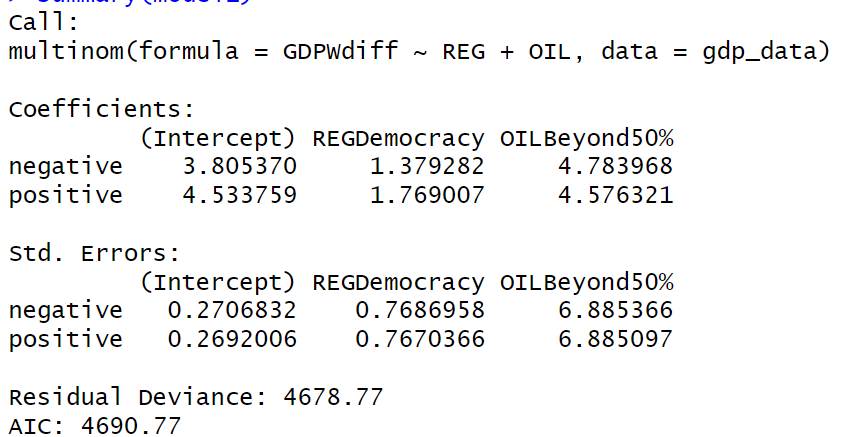
\includegraphics[width=0.7\textwidth]{Q1_1.png}\\
	Intercept coefficient: For GDPWdiff, the reference category is "negative" and the intercept coefficient is 3.805370. This indicates that, with other predictor variables remaining unchanged, the log adds of GDPWdiff in the negative category are approximately 3.805370 relative to the reference category.\\
	
	REGDemocracy coefficient: For the case where the REG variable belongs to the "Democracy" category, the REGDemocracy coefficient is 1.379282 relative to the "Non Democracy" category of the REG variable. This indicates that, while keeping other predictor variables constant, the logarithmic probability of GDPWdiff in the "positive" category is approximately 1.379282 compared to the reference category when REG is "Democracy".\\
	
	OILBeyond50\% coefficient: For cases where the OIL variable is in the "Beyond 50\%" category, the coefficient for OILBeyond50\% is 4.783968 relative to the "Below 50\%" category of the OIL variable. This indicates that, while keeping other predictor variables constant, the logarithmic probability of GDPWdiff in the negative category is approximately 4.783968 compared to the reference category when OIL is "Beyond 50\%".
	\\
	The standard error provides information about the accuracy of coefficient estimation. A smaller standard error indicates a more accurate estimation.\\
	The residual deviation measurement model measures the overall goodness of fit of the data. A smaller residual deviation value indicates a better fit with the observed data. AIC is a measure of the goodness of fit of a model, adjusted based on the number of predictive factors. The smaller the AIC value, the more suitable the model is.
	\\
	\lstinputlisting[language=R, firstline=69,lastline=73]{PS3.R} 
	\textbf{Result}:\\
	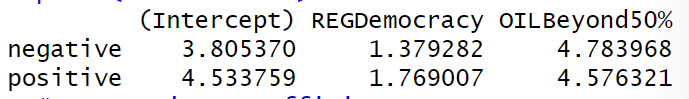
\includegraphics[width=0.7\textwidth]{Q1_4.png}\\
	
	For negative level GDPWdiff, the Intercept at the cut-off point is 3.81, and the coefficient of REGDemography is 1.379282\\
	The coefficient of OILBeyond50\% is 4.783968
	For the positive level of GDPWdiff, the Intercept at the cut-off point is 4.533759, the coefficient for REGDemocracy is 1.769007, and the coefficient for OILBeyond50\% is 4.576321
	\\
	\lstinputlisting[language=R, firstline=74,lastline=75]{PS3.R} 
	\textbf{Result}:\\
	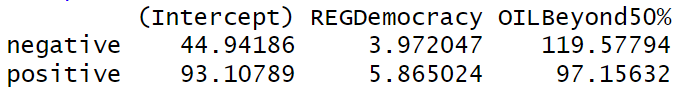
\includegraphics[width=0.7\textwidth]{Q1_2.png}\\
	1.Intercept (Negative to Positive): The exponentiated intercept of 44.94 indicates that when all other predictors are held constant, the odds of transitioning from the negative level to the positive level of GDPWdiff are approximately 44.94 times higher than remaining in the negative level, for observations with the reference categories of REG (Non-Democracy) and OIL (Below50\%).\\ 
	
	2.REGDemocracy (Negative to Positive): The exponentiated coefficient of 3.97 for REGDemocracy suggests that, holding OIL constant, the odds of transitioning from the negative level to the positive level of GDPWdiff are approximately 3.97 times higher for observations with a regime categorized as Democracy compared to Non-Democracy. \\
	
	3.OILBeyond50\% (Negative to Positive): The exponentiated coefficient of 119.58 for OILBeyond50\% implies that, when controlling for REG, the odds of transitioning from the negative level to the positive level of GDPWdiff are approximately 119.58 times higher for observations with oil production categorized as Beyond50\% compared to Below50\%.\\
	
	\item Construct and interpret an ordered multinomial logit with \texttt{GDPWdiff} as the outcome variable, including the estimated cutoff points and coefficients.
	\lstinputlisting[language=R, firstline=77,lastline=88]{PS3.R} 
	\textbf{Result}:\\
	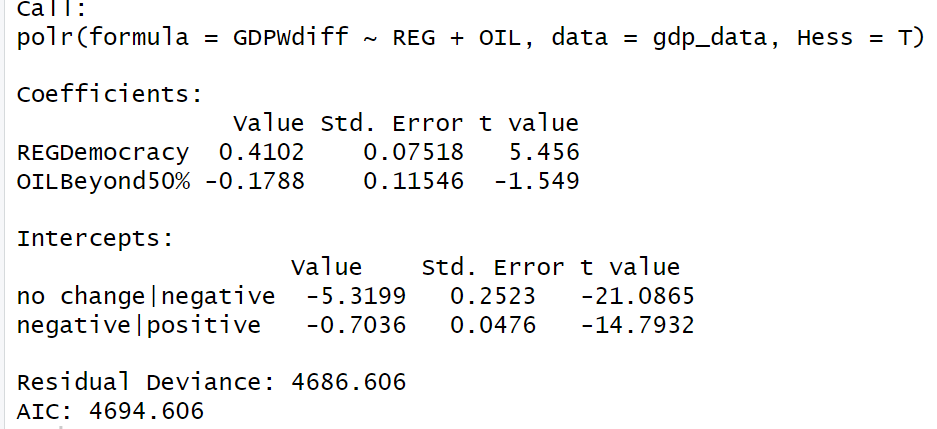
\includegraphics[width=0.7\textwidth]{Q1_3.png}\\
	In the results of this ordered multiple logistic regression model, the REGDemocracy coefficient is 0.4102, the standard error is 0.07518, and the t-value is 5.456. This indicates that when the REG variable changes from "Non Democracy" to "Democracy", the logarithmic probability of transitioning from lower GDPWdiff categories to higher GDPWdiff categories increases by 0.4102 units. A t-value of 5.456 indicates that this change is significant, as its absolute value is much greater than 1.96 (at a 95\% confidence level).\\
	
	The OILBeyond 50\% coefficient is -0.1788, the standard error is 0.11546, and the t-value is -1.549. When the OIL variable changed from "Below50\%" to "Beyond 50\%", the log adds for transitioning from higher GDPWdiff categories to lower GDPWdiff categories decreased by 0.1788 units. Although the t-value is -1.549, it is not significant as its absolute value is less than 1.96.\\
	
	The intercept represents the log adds for converting from one GDPWdiff class to another. The intercept from no change to negative category is -5.3199, which means that the log addresses for converting from no change to negative category are -5.3199. The intercept from negative to positive category is -0.7036, indicating that the log adds for transitioning from negative to positive category are -0.7036.
	\\
	\lstinputlisting[language=R, firstline=89,lastline=93]{PS3.R} 
	\textbf{Result}:\\
	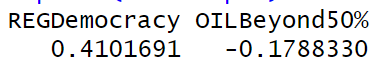
\includegraphics[width=0.4\textwidth]{Q1_5.png}\\
	The estimated value of the REGDemocracy coefficient is 0.4101691. This indicates that when the REG variable changes from "Non Democracy" to "Democracy", the log additions for transitioning from lower GDPWdiff categories to higher GDPWdiff categories increase by 0.4101691 units.
	The estimated value of the OILBeyond 50\% coefficient is -0.1788330. This indicates that when the OIL variable changes from "Below50\%" to "Beyond 50\%", the log adds for transitioning from higher GDPWdiff categories to lower GDPWdiff categories decrease by 0.1788330 units.
	\\
	
	
\end{enumerate}

\section*{Question 2} 
\vspace{.25cm}

\noindent Consider the data set \texttt{MexicoMuniData.csv}, which includes municipal-level information from Mexico. The outcome of interest is the number of times the winning PAN presidential candidate in 2006 (\texttt{PAN.visits.06}) visited a district leading up to the 2009 federal elections, which is a count. Our main predictor of interest is whether the district was highly contested, or whether it was not (the PAN or their opponents have electoral security) in the previous federal elections during 2000 (\texttt{competitive.district}), which is binary (1=close/swing district, 0="safe seat"). We also include \texttt{marginality.06} (a measure of poverty) and \texttt{PAN.governor.06} (a dummy for whether the state has a PAN-affiliated governor) as additional control variables. 

\begin{enumerate}
	\item [(a)]
	Run a Poisson regression because the outcome is a count variable. Is there evidence that PAN presidential candidates visit swing districts more? Provide a test statistic and p-value.
	\lstinputlisting[language=R, firstline=99,lastline=102]{PS3.R} 
	\textbf{Result}:\\
	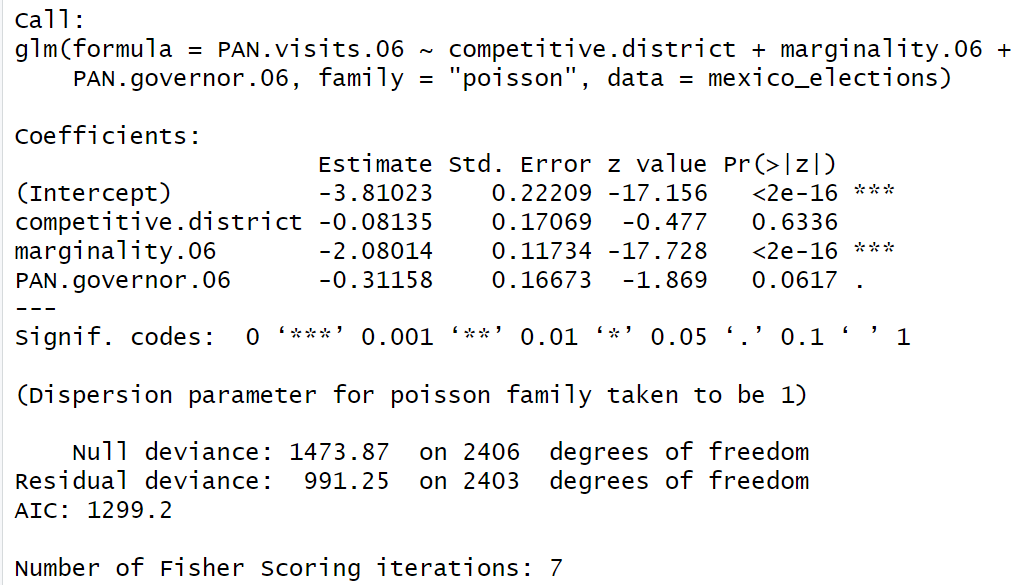
\includegraphics[width=0.7\textwidth]{Q2_1.png}\\
	According to the Poisson regression results above, the coefficient of the competitive. logistic variable is -0.08135, with a p-value of 0.6336. This means that, while keeping other variables constant, the relationship between competitive constituencies and PAN.visits.06 is not significant. Therefore, according to this model, there is no evidence to suggest that PAN presidential candidates are more inclined to visit competitive constituencies. The test statistic is -0.477.\\
	\item [(b)]
	Interpret the \texttt{marginality.06} and \texttt{PAN.governor.06} coefficients.\\
	\textbf{Result}:\\
	The margin. 06 coefficient is -2.08014, and its p-value is less than 2e-16, which is very significant. This indicates a significant negative correlation between marginalization (poverty level) and PAN.visits.06, while keeping other variables constant. The coefficient of PAN.governor.06 is -0.31158, with a p-value of 0.0617, which is close to the significance level of 0.05. This suggests that the relationship between the coefficient of whether the governor is a PAN party and PAN. visits.06 may be significant, while other variables remain unchanged, but further confirmation is needed.\\
	\item [(c)]
	Provide the estimated mean number of visits from the winning PAN presidential candidate for a hypothetical district that was competitive (\texttt{competitive.district}=1), had an average poverty level (\texttt{marginality.06} = 0), and a PAN governor (\texttt{PAN.governor.06}=1).
	\lstinputlisting[language=R, firstline=103,lastline=105]{PS3.R} 
	\textbf{Result}:\\
	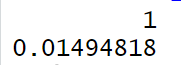
\includegraphics[width=0.3\textwidth]{Q2_2.png}\\
	 For hypothetical regions with competitive constituencies (competitive. district=1), average poverty level (marginal. 06=0), and PAN party governors (PAN. governor. 06=1), the average predicted number of visits by PAN presidential candidates is 0.0149.\\
\end{enumerate}

\end{document}
